\section{Background}

\subsection{Problem Statement}

\begin{frame}{}
  \begin{center}
    Why is this not about ANNS anymore?
  \end{center}
\end{frame}

\begin{frame}{}
  \begin{definition}[Random Sampling without Replacement]
    Given a data set \(X\), we uniformly pick \(k\) elements
    from \(X\) such that none repeat.
  \end{definition}

  Use cases:
  \begin{itemize}
    \item Splitting train-test data for ML 
    \item Subsampling for efficiency
  \end{itemize}
\end{frame}

\begin{frame}{Work-Span Model for Cost Analysis}
  \begin{definition}[Work]
    The \textit{work}, often denoted by \(W\), of a parallel algorithm is the 
    total number of operations done in the whole computation.
  \end{definition}

  \begin{definition}[Span]
    The \textit{span}, often denoted by \(S\), of a parallel algorithm is the
    longest chain of dependencies in a computation DAG.
  \end{definition}
\end{frame}

\begin{frame}{Work-Span Model for Cost Analysis Example}
  \begin{algorithm}[H]
    \caption{ParComp}
    \begin{algorithmic}
      \State{Compute \(A\) and \(B\) in parallel}
      \State{Compute \(C\)}
    \end{algorithmic}
  \end{algorithm}
  
  \(A\), \(B\), and \(C\) takes \(a, b\), and \(c\) operations respectively.
  \begin{itemize}
    \item Work is \(a + b + c\)
    \item Span is \(\max(a, b) + c\)
  \end{itemize}
\end{frame}

\subsection{Existing Algorithms}

\begin{frame}{Baseline: Pick and Remove}
  \begin{algorithm}[H]
    \caption{\textsc{PickAndRemove}}
  \begin{algorithmic}
    \Input{Data set \(X\), Sample size \(k\)}
    \Output{Sample \(S\) with \(|S| = k\)}
    \For{\(i = 1, 2, \ldots, k\)}
      \State{Pick \(x\) u.a.r. from \(X\)}
      \State{Add \(x\) to \(S\)}
      \State{Remove \(x\) from \(X\)}
    \EndFor
    \State{\Return{\(S\)}}
  \end{algorithmic}
  \end{algorithm}

  Sequential running time of \(\O(n)\).
\end{frame}

\begin{frame}{Improvement 1: Priority Sampling}
  \begin{algorithm}[H]
    \caption{\textsc{PrioritySample}}
  \begin{algorithmic}
    \Input{Data set \(X\), Sample size \(k\)}
    \Output{Sample with size \(k\)}

    \State{Assign priority from \(\Unif(0, 1)\) to each element
    of \(X\)}
    \State{\Return{\textsc{QuickSelect(\(X, k\))} using priority for comparison}}
  \end{algorithmic}
  \end{algorithm}

  Sequential running time of \(\O(n)\) w.h.p.\footnote{Probability at least \(1 -
  n^{-c}\) for constant \(c > 0\)}
\end{frame}

\begin{frame}{Improvement 1': Priority Sampling}
  \begin{algorithm}[H]
    \caption{\textsc{ParPrioritySample}}
  \begin{algorithmic}
    \Input{Data set \(X\), Sample size \(k\)}
    \Output{Sample with size \(k\)}

    \State{Assign priority from \(\Unif(0, 1)\) to each element
    of \(X\) in parallel}
    \State{\Return{\textsc{ParQuickSelect(\(X, k\))} using priority for comparison}}
  \end{algorithmic}
  \end{algorithm}

  Work is \(\O(n)\) and span is \(\O(\log^2 n)\).

  Performs pretty well when \(k \approx n\).
\end{frame}

% \begin{frame}{Recap: Quick Select}
%   \begin{algorithm}[H]
%     \caption{\textsc{QuickSelect}}
%   \begin{algorithmic}
%     \Input{Data set \(Y\), Sample size \(l\)}
%     \Output{Sample with size \(l\)}
%
%     \State{Pick \(p\) u.a.r. from \(Y\)}
%     \State{\(LE \gets\) elements of \(Y\) less than or equals to \(p\)}
%     \State{\(G \gets\) elements of \(Y\) greater than \(p\)}
%
%     \IIf{\(|LE| = k\)}{\Return{\(LE\)}}
%     \IElsIf{\(|LE| > k\)}{\Return{\textsc{QuickSelect(\(LE, l\))}}}
%     \IElse{\Return{\textsc{Concat(\(LE\), QuickSelect(\(G,
%     l - |LE|\)))}}}
%   \end{algorithmic}
%   \end{algorithm}
%
%   The parallel variant constructs \(LE\) \(G\) in parallel.
% \end{frame}

\begin{frame}{Improvement 2: Permutation Sampling}
  \begin{algorithm}[H]
    \caption{\textsc{PermutationSample}}
  \begin{algorithmic}
    \Input{Data set \(X\), Sample size \(k\)}
    \Output{Sample with size \(k\)}

    \State{Generate swap target \(H\) such that \(i \leq H[i] \leq n\)}
    \State{\textsc{Permute(\(X, H\))}}
    \State{\Return{\(X[{}:k]\)}}
  \end{algorithmic}
  \end{algorithm}

  \begin{algorithm}[H]
    \caption{\textsc{Permute} or Knuth Shuffle via Fisher-Yates}
  \begin{algorithmic}
    \Input{Data set \(X\), Swap target \(H\)}
    \For{\(i = 1, 2, \ldots, n\)}
      \State{\textsc{Swap(\(A[i], A[H[i]]\))}}
    \EndFor
  \end{algorithmic}
  \end{algorithm}
\end{frame}

\begin{frame}{Can we do better?}
  So far, existing algorithms run in \(\O(n)\)
  \begin{enumerate}
    \item When \(k \approx n\), doesn't really matter
    \item When \(k \ll n\), does too much work
  \end{enumerate}

  This project focuses on tackling the second case this using Permutation Sampling.
\end{frame}

\subsection{Improvements via Permutation Sampling}

\begin{frame}{Knuth Shuffle}
  One small issue: \textsc{Permute} is super sequential!

  \begin{algorithm}[H]
    \caption{\textsc{Permute} or Knuth Shuffle via Fisher-Yates}
    \begin{algorithmic}
      \Input{Data set \(X\), Swap target \(H\)}
      \For{\(i = 1, 2, \ldots, n\)}
        \State{\textsc{Swap(\(A[i], A[H[i]]\))}}
      \EndFor
    \end{algorithmic}
  \end{algorithm}
\end{frame}

% \begin{frame}{Knuth Shuffle}
%   \begin{figure}
%     \begin{center}
%       :: inserts Knuth Shuffle picture here ::
%     \end{center}
%     \caption{Example of Knuth Shuffle}\label{fig:knuth-shuffle-example}
%   \end{figure}
% \end{frame}

\begin{frame}{Parallel Knuth Shuffle}
  According to Shun et al. \cite{julian-parperm}, you can run Knuth Shuffle in
  parallel.

  \begin{figure}[ht]
    \begin{center}
      \includegraphics[width=0.60\textwidth]{julian-paper}
    \end{center}
    \caption{Shun et al. \cite{julian-parperm}}
  \end{figure}
\end{frame}

\begin{frame}{Parallel Knuth Shuffle}
  Useful results:
  \begin{enumerate}
    \item Swap target \(H\) can be converted into a Dependency Directed Acyclic
      Graph
    \item \(\O(1)\) \textit{readiness} detection gives \(\O(n)\) work and
      \(\O(\log n)\) span for Knuth Shuffle w.h.p.
    \item Parallel and sequential Knuth Shuffle gives same output using
      \textit{deterministic reservation}
  \end{enumerate}
\end{frame}

\begin{frame}{Parallel Knuth Shuffle}
  \begin{figure}
    \begin{center}
      \begin{subfigure}{0.45\textwidth}
        \vfill
        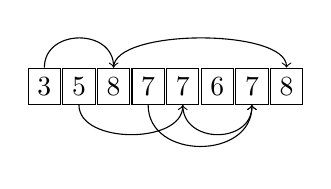
\begin{tikzpicture}[
          arr-elm/.style = {draw, rectangle, text centered, minimum size=0.5em}, 
          node distance = 1.25em
        ]
          \node[arr-elm] (1) {3};
          \node[arr-elm,right of=1] (2) {5};
          \node[arr-elm,right of=2] (3) {8};
          \node[arr-elm,right of=3] (4) {7};
          \node[arr-elm,right of=4] (5) {7};
          \node[arr-elm,right of=5] (6) {6};
          \node[arr-elm,right of=6] (7) {7};
          \node[arr-elm,right of=7] (8) {8};

          \draw[->] (1.north) .. controls +(up:5mm) and +(up:5mm) .. (3.north);
          \draw[->] (3.north) .. controls +(up:5mm) and +(up:5mm) .. (8.north);

          \draw[->] (2.south) .. controls +(down:5mm) and +(down:5mm) .. (5.south);
          \draw[->] (5.south) .. controls +(down:5mm) and +(down:5mm) .. (7.south);

          \draw[->] (4.south) .. controls +(down:7mm) and +(down:7mm) .. (7.south);
        \end{tikzpicture}
        \vfill
      \end{subfigure}
      \begin{subfigure}{0.45\textwidth}
        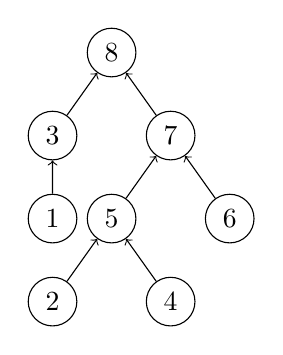
\begin{tikzpicture}[
            vtx/.style = {draw, circle},
            edge from parent/.style = {draw,<-},
            level/.style = {level distance = 3em}
          ]
          \node[vtx] {8}
            child { node[vtx] {3} child { node[vtx] {1} } }
            child { 
              node[vtx] {7}
              child { node[vtx] {5} 
                  child { node[vtx] {2} }
                  child { node[vtx] {4} }
                }
                child { node[vtx] {6} }
            }
          ;
        \end{tikzpicture}
      \end{subfigure}
    \end{center}
    \caption{DDAG constructed from \(H = [
      \underset{1}{3}, 
      \underset{2}{5}, 
      \underset{3}{8}, 
      \underset{4}{7}, 
      \underset{5}{7}, 
      \underset{6}{6}, 
      \underset{7}{7}, 
      \underset{8}{8} 
    ]\)}
  \end{figure}
\end{frame}

\begin{frame}{Parallel Knuth Shuffle}
  \begin{definition}[Ready]
    Step \(i\) is said to be \textit{ready} if every step that
    points to \(i\) in the DDAG has been processed.
  \end{definition}
\end{frame}

\begin{frame}{Parallel Knuth Shuffle}
  \begin{columns}
    \begin{column}{0.4\textwidth}
      \begin{figure}
        \begin{center}
          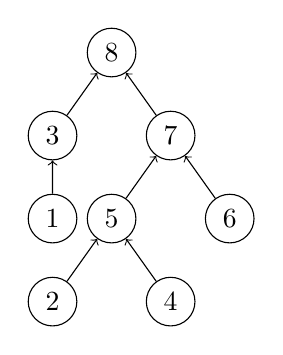
\begin{tikzpicture}[
              vtx/.style = {draw, circle},
              edge from parent/.style = {draw,<-},
              level/.style = {level distance = 3em}
            ]
            \node[vtx] {8}
              child { node[vtx] {3} 
                child { node[vtx] {1} } 
              }
              child { node[vtx] {7}
                child { node[vtx] {5} 
                  child { node[vtx] {2} }
                  child { node[vtx] {4} }
                }
                child { node[vtx] {6} }
              }
            ;
          \end{tikzpicture}
        \end{center}
        \caption{\(H = [
          \underset{1}{3}, 
          \underset{2}{5}, 
          \underset{3}{8}, 
          \underset{4}{7}, 
          \underset{5}{7}, 
          \underset{6}{6}, 
          \underset{7}{7}, 
          \underset{8}{8} 
        ]\)}
      \end{figure}
    \end{column}
    \begin{column}{0.6\textwidth}
      \begin{itemize}
        \item 5 is ready if 2 and 4 are processed
        \item 7 is ready if 5 and 6 are processed
        \item 3 is ready if 1 is processed
        \item 8 is ready if 3 and 7 are processed
      \end{itemize}
    \end{column}
  \end{columns}
\end{frame}

\begin{frame}{Parallel Knuth Shuffle}
  \begin{columns}
    \begin{column}{0.4\textwidth}
      \begin{figure}
        \begin{center}
          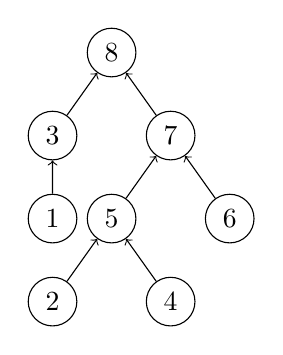
\begin{tikzpicture}[
              vtx/.style = {draw, circle},
              edge from parent/.style = {draw,<-},
              level/.style = {level distance = 3em}
            ]
            \node[vtx] {8}
              child { node[vtx] {3} 
                child { node[vtx] {1} } 
              }
              child { node[vtx] {7}
                child { node[vtx] {5} 
                  child { node[vtx] {2} }
                  child { node[vtx] {4} }
                }
                child { node[vtx] {6} }
              }
            ;
          \end{tikzpicture}
        \end{center}
        \caption{\(H = [
          \underset{1}{3}, 
          \underset{2}{5}, 
          \underset{3}{8}, 
          \underset{4}{7}, 
          \underset{5}{7}, 
          \underset{6}{6}, 
          \underset{7}{7}, 
          \underset{8}{8} 
        ]\)}
      \end{figure}
    \end{column}
    \begin{column}{0.6\textwidth}
      \begin{itemize}
        \item Readiness of 5 checked twice
        \item Readiness of 7 checked thrice
        \item Readiness of 3 checked twice
        \item Readiness of 8 checked 4 times
      \end{itemize}
    \end{column}
  \end{columns}
\end{frame}

\begin{frame}{Parallel Knuth Shuffle}
  \textit{Deterministic Reservation} is a framework by Blelloch et al. 
  \cite{blelloch-detreserve}
  \begin{itemize}
    \item For parallel algorithms whose dependency DAG is
      unique for each input under fork-join
      \begin{itemize}
        \item \textsc{MergeSort} has only one DDAG for one input
        \item \textsc{QuickSort} could have multiple DDAG for one input
          input
      \end{itemize}
    \item Ensure determinism despite different CPU scheduling
    \item Splits processing round into 2 phases: Reservation and Committing
  \end{itemize}
\end{frame}

\begin{frame}{Parallel Knuth Shuffle}
  Primitive from DR: \textsc{WriteMin(\(l, x\))}
  \begin{itemize}
    \item Writes \(\min(l_{\text{val}}, x)\) into memory location \(l\)
    \item Used to tackle race conditions
    \item Can be implemented with atomics
  \end{itemize}
\end{frame}
